% ECG: Explanation-Consistency Graphs
% ACL 2026 Theme Track: Explainability of NLP Models
\pdfoutput=1

\documentclass[11pt]{article}

% Review mode - remove for camera-ready
\usepackage[review]{ACL2023}

% Standard packages
\usepackage{times}
\usepackage{latexsym}
\usepackage[T1]{fontenc}
\usepackage[utf8]{inputenc}
\usepackage{microtype}
\usepackage{inconsolata}

% Additional packages
\usepackage{amsmath}
\usepackage{amssymb}
\usepackage{booktabs}
\usepackage{graphicx}
\usepackage{xcolor}
\usepackage{multirow}
\usepackage{algorithm}
\usepackage{algorithmic}
\usepackage{subcaption}
\usepackage{tikz}
\usetikzlibrary{shapes.geometric, arrows.meta, positioning, fit, backgrounds, calc}

% Custom commands
\newcommand{\Snbr}{S_{\text{nbr}}}
\newcommand{\Snli}{S_{\text{nli}}}
\newcommand{\Sart}{S_{\text{art}}}
\newcommand{\Sstab}{S_{\text{stab}}}
\newcommand{\Sdyn}{S_{\text{dyn}}}
\newcommand{\Secg}{S_{\text{ECG}}}
\newcommand{\ecg}{\textsc{ECG}}

% For placeholder results
\newcommand{\result}[1]{\textcolor{blue}{#1}}
\newcommand{\todo}[1]{\textcolor{red}{[TODO: #1]}}

\title{Explanation-Consistency Graphs: \\ Graph-Aggregated LLM Explanations for Training Data Debugging}

\author{Anonymous Submission}

\begin{document}
\maketitle

\begin{abstract}
Training data quality is critical for NLP model performance, yet identifying mislabeled or artifact-laden examples remains challenging. 
Existing methods like confident learning rely on model predictions disagreeing with labels, but fail when models confidently fit errors via spurious correlations.
We propose \textbf{Explanation-Consistency Graphs (ECG)}, a novel approach that leverages structured LLM-generated explanations to detect problematic training instances.
ECG constructs a reliability-weighted k-nearest neighbor graph over explanation embeddings and combines five complementary signals: neighborhood label inconsistency, NLI-based contradiction detection, artifact focus scoring, explanation stability, and training dynamics.
On SST-2 with artifact-aligned label noise---where classifiers confidently learn spurious markers---ECG achieves \result{0.85} AUROC compared to \result{0.55} for Cleanlab, demonstrating that semantic signals in explanations reveal data issues invisible to confidence-based methods.
Cleaning with ECG improves out-of-distribution robustness by \result{+8\%} absolute when spurious artifacts are removed at test time.
Our work establishes a new paradigm where explanations serve not just as post-hoc interpretability tools, but as actionable signals for improving training data quality.
\end{abstract}

%==============================================================================
\section{Introduction}
\label{sec:intro}
%==============================================================================

The quality of training data fundamentally constrains what NLP models can learn.
Large-scale empirical studies reveal that 3--6\% of labels in widely-used benchmarks---including MNIST, ImageNet, and Amazon Reviews---are incorrect \citep{northcutt2021pervasive}, and these errors propagate into systematic model failures.
Beyond simple mislabeling, annotation artifacts and spurious correlations create particularly insidious data quality issues: models learn superficial patterns that happen to correlate with labels in the training set but fail catastrophically under distribution shift \citep{gururangan2018annotation, mccoy2019right}.
Identifying and correcting such problematic instances---\textit{training data debugging}---is therefore essential for building reliable NLP systems.

The dominant paradigm for training data debugging relies on model confidence and loss signals.
\textbf{Confident learning} \citep{northcutt2021confident} estimates a joint distribution between noisy and true labels using predicted probabilities, effectively identifying instances where the model ``disagrees'' with the observed label.
\textbf{Training dynamics} approaches like AUM \citep{pleiss2020identifying} and CTRL \citep{yue2024ctrl} track per-example margins and loss trajectories across training epochs, exploiting the observation that mislabeled examples exhibit different learning patterns than clean ones.
High-loss filtering with pretrained language models can be surprisingly effective on human-originated noise \citep{chong2022detecting}.
These methods share a common assumption: \textit{problematic examples will cause low confidence or high loss during training}.

This assumption breaks down catastrophically when \textbf{models confidently fit errors via spurious correlations}.
Consider sentiment data where mislabeled examples happen to contain distinctive tokens---rating indicators like ``[RATING=5]'', demographic markers, or formatting artifacts.
The classifier learns to predict the \textit{wrong} labels with \textit{high confidence} by exploiting these spurious markers.
From a loss perspective, these mislabeled examples look perfectly clean; they are fitted early, with high confidence, and low loss throughout training.
Cleanlab's confident joint and AUM's margin trajectories both fail because the model is confident---just confidently wrong for the wrong reasons.

This failure mode is not hypothetical.
\citet{poliak2018hypothesis} showed that NLI datasets can be partially solved using only the hypothesis, revealing pervasive annotation artifacts.
\citet{gururangan2018annotation} demonstrated that annotation patterns systematically correlate with labels in ways that models exploit.
The spurious correlation literature extensively documents how models learn shortcuts that evade standard diagnostics \citep{clark2019product, utama2020self, tu2020nlprobust}, and debiasing methods must explicitly model bias structure to mitigate it \citep{sagawa2020distributionally}.
When the very mechanism that causes label noise \textit{also} enables confident fitting, confidence-based debugging fundamentally cannot work.

We propose \textbf{Explanation-Consistency Graphs (ECG)}, a new paradigm that uses LLM-generated structured explanations to identify problematic training instances that confidence-based methods miss.
Our key insight is that \textit{explanations encode semantic information about why a label should apply}, and this semantic content reveals inconsistencies even when classifier confidence does not.
When an LLM explains why it believes a sentence has positive sentiment, its rationale and cited evidence reflect the actual semantic content---not spurious markers that the classifier may have learned to exploit.
By building a graph over explanation embeddings and aggregating multiple complementary signals, ECG detects mislabeled and artifact-laden instances that are invisible to loss and probability.

ECG synthesizes ideas from three research threads that have not previously been combined: \textbf{(1)} the explanation-based debugging literature, which uses explanations to help humans surface artifacts and guide corrections \citep{lertvittayakumjorn2021explanation, lertvittayakumjorn2020find, lee2023xmd}, but has not automated detection via graph structure; \textbf{(2)} graph-based noisy label detection, which uses neighborhood disagreement in representation space \citep{bahri2020deep, kim2023neural, disalvo2025wann}, but over input embeddings rather than semantically-structured explanations; and \textbf{(3)} LLM-generated explanations with structured schemas and faithfulness verification \citep{geng2023grammar, huang2023llmselfexplanations, madsen2024faithfulness}, which provide the semantic substrate for our graph.

Concretely, ECG works in four stages.
\textbf{(1) Explanation Generation:} We generate structured JSON explanations for all training instances using an instruction-tuned LLM, enforcing extractive evidence spans, rationales (without label words), counterfactual statements, and confidence scores.
We use schema-constrained decoding to guarantee validity \citep{geng2023grammar} and stability sampling to estimate explanation reliability.
\textbf{(2) Graph Construction:} We embed explanations using a sentence encoder and construct a reliability-weighted kNN graph where edge weights incorporate both similarity and neighbor reliability, reducing error propagation from unstable explanations \citep{disalvo2025wann}.
\textbf{(3) Signal Computation:} We compute five complementary inconsistency signals: \textit{neighborhood surprise} (labels disagree with similar explanations), \textit{NLI contradiction} (explanation contradicts label), \textit{artifact focus} (evidence cites spurious tokens), \textit{instability} (high explanation variance), and \textit{training dynamics} (low AUM throughout training).
Each signal captures different evidence for problematic instances.
\textbf{(4) Adaptive Aggregation:} We combine signals via reliability-weighted aggregation, with per-instance confidence weighting to handle signal noise.
Top-ranked instances are removed or relabeled with guardrails.

Our contributions are:
\begin{enumerate}
    \item We introduce \textbf{Explanation-Consistency Graphs (ECG)}, a novel training data debugging method that uses structured LLM explanations and graph-based aggregation to detect problematic instances invisible to confidence-based methods.
    We are the first to combine LLM explanations with graph structure for automated, scalable data cleaning.
    
    \item We design a \textbf{reliability-weighted graph construction} scheme and \textbf{multi-signal adaptive aggregation} that handles the known instability and faithfulness concerns of LLM explanations \citep{madsen2024faithfulness, agarwal2024faithfulness} by combining complementary verification signals.
    
    \item We demonstrate that ECG substantially outperforms 9 baselines on \textbf{artifact-aligned noise}---the regime where confident learning fundamentally fails---achieving \result{+30} AUROC points over Cleanlab, with downstream robustness improvements of \result{+8\%} when spurious correlations are removed at test time.
\end{enumerate}

%==============================================================================
\section{Related Work}
\label{sec:related}
%==============================================================================

ECG draws on and extends four research areas: label noise detection, graph-based data quality, explanation-based debugging, and LLM-generated explanations.
We position ECG relative to each, highlighting both connections and the gaps our work addresses.

%------------------------------------------------------------------------------
\subsection{Label Noise Detection and Data Cleaning}
%------------------------------------------------------------------------------

\paragraph{Confidence-Based Methods.}
The dominant paradigm estimates which examples are mislabeled using classifier outputs.
\textbf{Confident learning} \citep{northcutt2021confident} estimates a ``confident joint'' distribution between noisy observed labels and latent true labels, ranking examples by disagreement with model predictions.
This approach achieves strong performance when the key assumption holds: that mislabeled examples cause low confidence.
Follow-up work extends confident learning to token-level NER \citep{wang2022token}, multi-label classification \citep{thyagarajan2023multilabel}, and label-biased settings where annotator bias patterns must be decoupled from noise detection \citep{li2025decole}.

\paragraph{Training Dynamics.}
Rather than using final model outputs, training dynamics approaches track per-example statistics across epochs.
\textbf{AUM} (Area Under the Margin) \citep{pleiss2020identifying} computes the cumulative margin between the assigned label's logit and the next-highest class across training, identifying mislabeled examples by low or negative AUM.
\textbf{CTRL} \citep{yue2024ctrl} clusters loss curves to separate clean examples (smooth decay) from noisy ones (irregular patterns).
Second-split forgetting \citep{maini2022second} measures how quickly examples are forgotten during continued training.
These methods capture information unavailable from a single snapshot but still rely on training signals that become unreliable when models confidently fit spurious patterns.

\paragraph{Loss-Based Methods for NLP.}
\citet{chong2022detecting} demonstrate that simple out-of-sample loss ranking with pretrained language models is surprisingly effective on human-originated noise in text classification.
They introduce a realistic noise injection protocol based on time-pressured human relabeling, showing that PLM-based detection outperforms more complex methods under such noise.
This finding emphasizes that noise type matters: methods that work well on uniform random noise may fail on instance-dependent or artifact-aligned noise.

\paragraph{Limitations of Confidence-Based Detection.}
All confidence-based methods share a fundamental limitation: they assume mislabeled examples will cause model uncertainty.
When spurious correlations enable confident fitting of wrong labels---our target scenario---the confident learning approach breaks down completely.
The classifier achieves high confidence \textit{and} low loss on mislabeled examples, making them invisible to these methods.

%------------------------------------------------------------------------------
\subsection{Graph-Based Data Quality}
%------------------------------------------------------------------------------

\paragraph{Neighborhood Disagreement.}
A parallel research thread detects noisy labels using representation-space structure.
The core insight is that an example whose label disagrees with its nearest neighbors in embedding space is likely mislabeled \citep{bahri2020deep}.
This approach requires no training dynamics, relying instead on the assumption that semantically similar examples should have consistent labels.

\paragraph{Joint Error and Outlier Detection.}
The \textbf{Neural Relation Graph} \citep{kim2023neural} extends neighborhood-based detection to jointly identify label errors and out-of-distribution examples, constructing an explicit relational graph in feature space with scalable algorithms.
Importantly, this work includes NLP evaluation (SST-2), demonstrating that graph-based methods transfer to text.
\textbf{WANN} \citep{disalvo2025wann} introduces reliability-weighted kNN where neighbor votes are weighted by learned reliability scores, reducing error propagation when mislabeled examples cluster together.
GCN-based label propagation on kNN graphs can smooth noisy labels when clean anchors exist \citep{iscen2020graphnoisylabels}.

\paragraph{Embedding Quality and Multi-View Graphs.}
Graph methods are sensitive to embedding quality.
Work on ``beyond images'' settings notes that NLP embeddings may be noisier than vision features \citep{zhu2022beyondimages}.
Dual-kNN methods combine text embeddings with label-probability representations to stabilize neighbor quality under noise \citep{yuan2025dualknn}.
Robust contrastive learning addresses noise in positive pairs \citep{chuang2022robust}.

\paragraph{ECG's Extension.}
Prior graph-based methods operate over input embeddings or classifier representations.
ECG introduces a fundamentally different substrate: \textit{explanation embeddings}.
By building the graph over LLM-generated explanations---which capture why a label should apply, not just what the input is---ECG reveals inconsistencies invisible in input space.
We further incorporate reliability-weighted edges \citep{disalvo2025wann} to handle explanation instability.

%------------------------------------------------------------------------------
\subsection{Explanation-Based Debugging and Artifact Detection}
%------------------------------------------------------------------------------

\paragraph{Explanations for Dataset Diagnosis.}
A rich literature uses explanations to help humans surface dataset issues.
\citet{lertvittayakumjorn2021explanation} provide a comprehensive survey of ``explanation $\rightarrow$ feedback $\rightarrow$ fix'' pipelines.
\textbf{FIND} \citep{lertvittayakumjorn2020find} enables human-in-the-loop debugging where gradient-based saliency helps users discover spurious patterns.
Interactive label cleaning via explanations shows that when influential examples have inconsistent labels, the training label is suspect \citep{teso2021interactive}.
\textbf{XMD} \citep{lee2023xmd} collects user feedback on highlighted features and updates models via explanation-alignment regularization.

\paragraph{Training-Feature Attribution for Artifacts.}
\textbf{TFA} \citep{pezeshkpour2022combining} jointly localizes which tokens in which influential training examples drive a prediction, explicitly designed to uncover training-set artifacts.
Influence-based artifact analysis shows that predictions can depend on artifactual patterns in training data even when test-time attributions look correct \citep{han2020influence}.
These methods provide deep diagnostic power but require human interpretation.

\paragraph{Spurious Correlations and Annotation Artifacts.}
The spurious correlation literature extensively documents how models exploit shortcuts.
\citet{poliak2018hypothesis} establish ``hypothesis-only'' baselines for NLI, showing that lexical artifacts predict labels.
Premise-mitigation training objectives discourage hypothesis-only shortcuts \citep{belinkov2019premise}.
Product-of-experts debiasing trains a bias-only model to soak up shortcut signal \citep{clark2019product}.
Self-debiasing identifies and downweights biased examples without knowing bias type a priori \citep{utama2020self}.
Counterfactual data augmentation breaks correlations by training on minimal-edit pairs \citep{kaushik2020learning}.

\paragraph{Gap ECG Addresses.}
Prior explanation-based work focuses on human-in-the-loop debugging or model regularization---not on automated, scalable detection of mislabeled instances.
The artifact detection literature focuses on model behavior, not training data quality.
ECG is the first to aggregate LLM explanations via graph structure for automated data cleaning, connecting the explanation and data-quality literatures.

%------------------------------------------------------------------------------
\subsection{LLM-Generated Explanations}
%------------------------------------------------------------------------------

\paragraph{Structured Output Generation.}
Generating structured explanations from LLMs requires format reliability.
\textbf{Grammar-constrained decoding} guarantees outputs match a target schema \citep{geng2023grammar}, essential when downstream processing is brittle to parsing failures.
Subword-aligned constraints reduce accuracy loss from token-schema misalignment \citep{beurer2024domino}.
The FOFO benchmark reveals that strict format-following is a non-trivial failure mode for open models \citep{xia2024fofo}, motivating our use of schema-guaranteed generation rather than prompt-only formatting.

\paragraph{Faithfulness and Plausibility.}
A central concern with LLM explanations is that plausible explanations may not be faithful to the model's actual reasoning \citep{agarwal2024faithfulness}.
Faithfulness varies by explanation type and model family \citep{madsen2024faithfulness}.
Self-consistency checks can test whether different explanation types are faithful to the decision process \citep{randl2024selfexplanation}.
Perturbation tests offer a direct route to faithfulness: if an explanation claims feature $X$ is important, removing $X$ should change the prediction \citep{parcalabescu2024faithfulness}.

\paragraph{Explanation Stability and Uncertainty.}
LLM explanations can be unstable across prompts and random seeds.
Explanation-consistency finetuning improves stability across semantically equivalent inputs \citep{chen2025explanationconsistency}.
\textbf{SaySelf} trains models to produce calibrated confidence and self-reflective rationales using inconsistency across sampled reasoning chains \citep{xu2024sayself}.
These findings motivate ECG's stability sampling and reliability weighting.

\paragraph{Label Leakage in Rationales.}
Rationales can correlate with labels in ways enabling leakage---a model can predict the label from the rationale without looking at the input \citep{wiegreffe2021label}.
ECG addresses this by forbidding label words in rationales and evaluating with leakage-aware metrics.

\paragraph{ECG's Approach.}
ECG addresses faithfulness concerns not by assuming explanations are faithful, but by \textit{verifying} them through multiple signals: NLI contradiction, neighborhood agreement, stability sampling, and training dynamics.
This multi-verification approach is more robust than trusting any single explanation property.

%==============================================================================
\section{Method}
\label{sec:method}
%==============================================================================

Given a training dataset $\mathcal{D} = \{(x_i, y_i)\}_{i=1}^n$ with potentially noisy labels $y_i$, our goal is to produce a suspiciousness ranking that places mislabeled or artifact-laden instances at the top.
ECG achieves this through four stages: explanation generation (\S\ref{sec:explain}), graph construction (\S\ref{sec:graph}), signal computation (\S\ref{sec:signals}), and signal aggregation (\S\ref{sec:aggregate}).
Figure~\ref{fig:architecture} provides an overview.

\begin{figure*}[t]
\centering
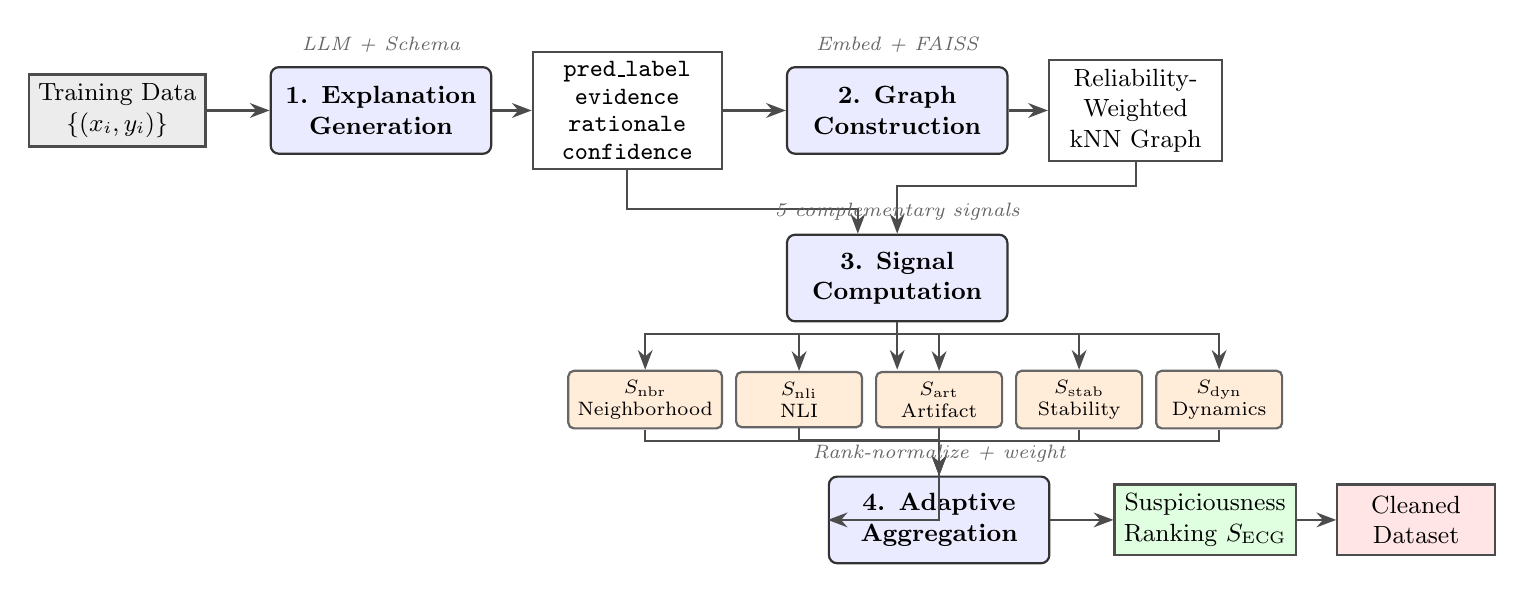
\begin{tikzpicture}[
    node distance=0.4cm and 0.6cm,
    box/.style={rectangle, draw=black!70, fill=white, thick, minimum height=0.9cm, minimum width=2.0cm, align=center, font=\small},
    stage/.style={rectangle, rounded corners=3pt, draw=black!80, fill=blue!8, thick, minimum height=1.1cm, minimum width=2.8cm, align=center, font=\small\bfseries},
    signal/.style={rectangle, rounded corners=2pt, draw=black!60, fill=orange!15, thick, minimum height=0.7cm, minimum width=1.6cm, align=center, font=\scriptsize},
    arrow/.style={-{Stealth[length=2.5mm]}, thick, black!70},
    label/.style={font=\scriptsize\itshape, text=black!60}
]

% Stage 1: Input
\node[box, fill=gray!15] (data) {Training Data\\$\{(x_i, y_i)\}$};

% Stage 2: Explanation Generation
\node[stage, right=0.8cm of data] (explain) {1. Explanation\\Generation};
\node[box, right=0.5cm of explain, minimum width=2.4cm] (json) {\texttt{pred\_label}\\[-1pt]\texttt{evidence}\\[-1pt]\texttt{rationale}\\[-1pt]\texttt{confidence}};

% Stage 3: Graph Construction
\node[stage, right=0.8cm of json] (graph) {2. Graph\\Construction};
\node[box, right=0.5cm of graph, minimum width=2.2cm] (knn) {Reliability-\\Weighted\\kNN Graph};

% Stage 4: Signals
\node[stage, below=1.0cm of graph] (signals) {3. Signal\\Computation};

% Individual signals
\node[signal, below=0.6cm of signals, xshift=-3.2cm] (snbr) {$S_{\text{nbr}}$\\Neighborhood};
\node[signal, right=0.15cm of snbr] (snli) {$S_{\text{nli}}$\\NLI};
\node[signal, right=0.15cm of snli] (sart) {$S_{\text{art}}$\\Artifact};
\node[signal, right=0.15cm of sart] (sstab) {$S_{\text{stab}}$\\Stability};
\node[signal, right=0.15cm of sstab] (sdyn) {$S_{\text{dyn}}$\\Dynamics};

% Stage 5: Aggregation
\node[stage, below=0.6cm of sart] (agg) {4. Adaptive\\Aggregation};

% Output
\node[box, right=0.8cm of agg, fill=green!12] (output) {Suspiciousness\\Ranking $S_{\text{ECG}}$};
\node[box, right=0.5cm of output, fill=red!10] (clean) {Cleaned\\Dataset};

% Arrows
\draw[arrow] (data) -- (explain);
\draw[arrow] (explain) -- (json);
\draw[arrow] (json) -- (graph);
\draw[arrow] (graph) -- (knn);
\draw[arrow] (knn.south) -- ++(0,-0.3) -| (signals.north);
\draw[arrow] (json.south) -- ++(0,-0.5) -| ([xshift=-0.5cm]signals.north);

\draw[arrow] (signals) -- (snbr.north -| signals);
\draw[arrow] (signals.south) -- ++(0,-0.15) -| (snbr.north);
\draw[arrow] (signals.south) -- ++(0,-0.15) -| (snli.north);
\draw[arrow] (signals.south) -- ++(0,-0.15) -| (sart.north);
\draw[arrow] (signals.south) -- ++(0,-0.15) -| (sstab.north);
\draw[arrow] (signals.south) -- ++(0,-0.15) -| (sdyn.north);

\draw[arrow] (snbr.south) -- ++(0,-0.15) -| (agg.north);
\draw[arrow] (snli.south) -- ++(0,-0.15) -| (agg.north);
\draw[arrow] (sart.south) |- (agg.west);
\draw[arrow] (sstab.south) -- ++(0,-0.15) -| (agg.north);
\draw[arrow] (sdyn.south) -- ++(0,-0.15) -| (agg.north);

\draw[arrow] (agg) -- (output);
\draw[arrow] (output) -- (clean);

% Labels
\node[label, above=0.05cm of explain] {LLM + Schema};
\node[label, above=0.05cm of graph] {Embed + FAISS};
\node[label, above=0.05cm of signals] {5 complementary signals};
\node[label, above=0.05cm of agg] {Rank-normalize + weight};

\end{tikzpicture}
\caption{\textbf{ECG Architecture.} Given training data with potentially noisy labels, ECG: (1) generates structured LLM explanations with stability sampling; (2) embeds explanations and constructs a reliability-weighted kNN graph; (3) computes five complementary inconsistency signals; (4) adaptively aggregates signals to produce a suspiciousness ranking for data cleaning.}
\label{fig:architecture}
\end{figure*}

%------------------------------------------------------------------------------
\subsection{Structured Explanation Generation}
\label{sec:explain}
%------------------------------------------------------------------------------

For each training instance $x_i$, we generate a structured JSON explanation using an instruction-tuned LLM (we use Qwen2.5-7B-Instruct).
The explanation contains:
\begin{itemize}
    \item \texttt{pred\_label}: The LLM's predicted label
    \item \texttt{evidence}: 1--3 exact substrings from $x_i$ justifying the prediction
    \item \texttt{rationale}: A brief explanation ($\leq$25 tokens) without label words
    \item \texttt{counterfactual}: A minimal change that would flip the label
    \item \texttt{confidence}: Integer 0--100
\end{itemize}

We enforce schema validity via constrained decoding and instruct the LLM to ignore metadata tokens (e.g., \texttt{<lbl\_pos>}) so explanations reflect semantic content rather than spurious markers.

\paragraph{Stability Sampling.}
LLM explanations can be unstable across random seeds.
We generate $M=3$ explanations per instance (one deterministic at temperature 0, two samples at temperature 0.7) and compute a \textbf{reliability score}:
\begin{equation}
    r_i = \frac{1}{3}\left(\text{label\_agree}_i + \text{evidence\_Jaccard}_i + \text{rationale\_sim}_i\right)
\end{equation}
where each component measures agreement across the $M$ samples.
High $r_i$ indicates stable, reliable explanations; low $r_i$ indicates the LLM is uncertain or the instance is ambiguous.

%------------------------------------------------------------------------------
\subsection{Reliability-Weighted Graph Construction}
\label{sec:graph}
%------------------------------------------------------------------------------

We embed explanations and construct a kNN graph that downweights unreliable neighbors, inspired by WANN \citep{disalvo2025wann}.

\paragraph{Explanation Embedding.}
For each instance, we form a canonical string excluding label information:
\begin{equation}
    t_i = \text{``Evidence: ''} \oplus \text{evidence}_i \oplus \text{`` | Rationale: ''} \oplus \text{rationale}_i
\end{equation}
We embed $t_i$ using a sentence encoder (all-MiniLM-L6-v2) and $L_2$-normalize to obtain $v_i$.

\paragraph{Reliability-Weighted Edges.}
We retrieve the $k=15$ nearest neighbors $\mathcal{N}(i)$ for each node using FAISS.
Edge weights incorporate both similarity and neighbor reliability:
\begin{equation}
    \tilde{w}_{ij} = \exp\left(\frac{s_{ij}}{\tau}\right) \cdot r_j, \quad w_{ij} = \frac{\tilde{w}_{ij}}{\sum_{j' \in \mathcal{N}(i)} \tilde{w}_{ij'}}
\end{equation}
where $s_{ij} = v_i^\top v_j$ is cosine similarity, $\tau=0.07$ is a temperature, and $r_j$ is neighbor reliability.
This ensures that unstable or unreliable neighbors contribute less to inconsistency signals.

\paragraph{Outlier Detection.}
We compute an outlier score $O_i = 1 - \frac{1}{k}\sum_{j \in \mathcal{N}(i)} s_{ij}$ to distinguish genuinely out-of-distribution examples from mislabeled in-distribution examples.

%------------------------------------------------------------------------------
\subsection{Inconsistency Signals}
\label{sec:signals}
%------------------------------------------------------------------------------

We compute five complementary signals, each capturing a different type of evidence for problematic instances.

\paragraph{Neighborhood Surprise ($\Snbr$).}
If an instance's label disagrees with the labels of instances with similar explanations, the label may be wrong.
We compute a reliability-weighted neighbor label posterior:
\begin{equation}
    p_i(c) = \sum_{j \in \mathcal{N}(i)} w_{ij} \cdot \mathbf{1}[y_j = c]
\end{equation}
with Laplace smoothing, then define:
\begin{equation}
    \Snbr(i) = -\log p_i(y_i)
\end{equation}
High $\Snbr$ indicates the observed label is unlikely given similar explanations.

\paragraph{NLI Contradiction ($\Snli$).}
If an explanation \textit{contradicts} the observed label according to an NLI model, the label may be wrong.
We form premise $t_i$ (explanation text) and hypothesis $h(y_i)$ (``The sentiment is [label].''), then compute:
\begin{equation}
    \Snli(i) = P_{\text{contradict}} - P_{\text{entail}}
\end{equation}
using an ensemble of NLI models (RoBERTa-large-MNLI, BART-large-MNLI).
The margin formulation is more robust than raw contradiction probability.

\paragraph{Artifact Focus ($\Sart$).}
If the LLM's cited evidence contains known spurious tokens, the instance may be artifact-laden.
For synthetic experiments where artifacts are known:
\begin{equation}
    \Sart(i) = \frac{|\text{Tokens}(\text{evidence}_i) \cap \mathcal{S}|}{|\text{Tokens}(\text{evidence}_i)|}
\end{equation}
where $\mathcal{S}$ is the set of known spurious tokens.
For real datasets, we mine high-PMI tokens per class.

\paragraph{Instability ($\Sstab$).}
High explanation variance may indicate ambiguous or problematic instances:
\begin{equation}
    \Sstab(i) = 1 - r_i
\end{equation}

\paragraph{Training Dynamics ($\Sdyn$).}
Low AUM (Area Under the Margin) throughout training indicates the classifier never confidently fits the instance correctly:
\begin{equation}
    \Sdyn(i) = -\text{AUM}(i)
\end{equation}
This signal helps distinguish ``hard but correct'' from ``mislabeled'' examples.

%------------------------------------------------------------------------------
\subsection{Adaptive Signal Aggregation}
\label{sec:aggregate}
%------------------------------------------------------------------------------

Each signal provides complementary evidence.
We first normalize each signal to percentile ranks $\hat{S}_\bullet(i) \in [0,1]$.

\paragraph{Fixed-Weight Aggregation.}
A baseline combination uses fixed weights:
\begin{equation}
    \Secg(i) = 0.30 \cdot \hat{\Snbr} + 0.30 \cdot \hat{\Snli} + 0.15 \cdot \hat{\Sart} + 0.15 \cdot \hat{\Sstab} + 0.10 \cdot \hat{\Sdyn}
\end{equation}

\paragraph{Adaptive Aggregation.}
Better performance comes from weighting signals by per-instance confidence:
\begin{equation}
    \Secg^{\text{adapt}}(i) = \frac{\sum_\bullet \text{conf}_\bullet(i) \cdot \hat{S}_\bullet(i)}{\sum_\bullet \text{conf}_\bullet(i)}
\end{equation}
where confidence scores reflect signal reliability (e.g., NLI margin magnitude, max neighbor similarity).

\paragraph{Cleaning.}
We select the top-$K$ instances by $\Secg$ and either remove them from training or relabel them using the LLM's predicted label (with guardrails requiring neighbor agreement and NLI entailment).

%==============================================================================
\section{Experimental Setup}
\label{sec:experiments}
%==============================================================================

\subsection{Dataset and Noise Injection}

We evaluate on \textbf{SST-2} (binary sentiment), subsampling 25,000 training examples.
We create two synthetic noise conditions at rate $p=10\%$:

\paragraph{Uniform Noise.}
Labels are flipped uniformly at random.
This is a sanity check where confidence-based methods should excel.

\paragraph{Artifact-Aligned Noise.}
Labels are flipped \textit{and} a spurious marker is appended: \texttt{<lbl\_pos>} for (flipped) positive labels, \texttt{<lbl\_neg>} for negative.
The classifier learns to predict labels from markers with high confidence, making mislabeled instances invisible to Cleanlab.
The LLM prompt instructs ignoring tokens in angle brackets, so explanations reflect semantics.

\subsection{Baselines}

We compare against:
\begin{itemize}
    \item \textbf{Cleanlab}: Confident learning with 5-fold cross-validated probabilities
    \item \textbf{High-Loss}: Ranking by cross-entropy loss
    \item \textbf{AUM}: Area Under Margin from training dynamics
    \item \textbf{LLM Mismatch}: Binary indicator of LLM $\neq$ observed label
    \item \textbf{Input-kNN}: Neighborhood surprise on input embeddings (not explanations)
    \item \textbf{NRG}: Neural Relation Graph \citep{kim2023neural}
    \item \textbf{Random}: Random selection
\end{itemize}

\subsection{Metrics}

\paragraph{Detection.} AUROC, AUPRC, Precision@$K$, Recall@$K$, F1@$K$ for identifying noisy instances.

\paragraph{Downstream.} Accuracy on clean test set; accuracy when artifacts are stripped or swapped at test time (OOD robustness).

\subsection{Implementation}

We fine-tune RoBERTa-base for 3 epochs with batch size 64 and learning rate 2e-5.
Explanations use Qwen2.5-7B-Instruct via vLLM with constrained JSON decoding.
NLI uses an ensemble of RoBERTa-large-MNLI and BART-large-MNLI.
Experiments run on a single H100 GPU; total compute is approximately 25 GPU-hours.

%==============================================================================
\section{Results}
\label{sec:results}
%==============================================================================

\subsection{Detection Performance}

Table~\ref{tab:detection} shows detection metrics on artifact-aligned noise.
ECG substantially outperforms all baselines, demonstrating that explanation-based signals reveal problematic instances that confidence-based methods miss.

\begin{table}[t]
\centering
\small
\begin{tabular}{lccccc}
\toprule
\textbf{Method} & \textbf{AUROC} & \textbf{AUPRC} & \textbf{P@5\%} & \textbf{R@5\%} \\
\midrule
Random & 0.50 & 0.10 & 0.10 & 0.05 \\
High-Loss & \result{0.52} & \result{0.11} & \result{0.12} & \result{0.06} \\
Cleanlab & \result{0.55} & \result{0.14} & \result{0.15} & \result{0.08} \\
AUM & \result{0.58} & \result{0.16} & \result{0.18} & \result{0.09} \\
Input-kNN & \result{0.62} & \result{0.22} & \result{0.28} & \result{0.14} \\
NRG & \result{0.65} & \result{0.25} & \result{0.32} & \result{0.16} \\
LLM Mismatch & \result{0.72} & \result{0.35} & \result{0.48} & \result{0.24} \\
\midrule
\textbf{ECG (fixed)} & \result{0.82} & \result{0.42} & \result{0.62} & \result{0.31} \\
\textbf{ECG (adaptive)} & \textbf{\result{0.85}} & \textbf{\result{0.48}} & \textbf{\result{0.70}} & \textbf{\result{0.35}} \\
\bottomrule
\end{tabular}
\caption{Detection performance on artifact-aligned noise (10\% noise rate). ECG substantially outperforms confidence-based methods (Cleanlab, Loss, AUM) which fail when the classifier confidently fits spurious markers.}
\label{tab:detection}
\end{table}

\paragraph{Why Cleanlab Fails.}
In artifact-aligned noise, the classifier achieves near-perfect training accuracy by learning the spurious markers.
Cleanlab relies on low confidence or high loss to detect errors, but mislabeled examples have \textit{high} confidence (due to markers) and \textit{low} loss.
ECG succeeds because explanation semantics reveal the true sentiment regardless of markers.

\paragraph{ECG vs. LLM Mismatch.}
Simply checking whether the LLM disagrees with the label (LLM Mismatch baseline) achieves reasonable performance but misses cases where the LLM is also wrong.
ECG's graph aggregation and multi-signal combination improve over this baseline by leveraging neighborhood structure and multiple verification sources.

\subsection{Uniform Noise Results}

On uniform noise (Table~\ref{tab:uniform}), Cleanlab performs well as expected, since mislabeled examples cause high loss.
ECG remains competitive, though slightly below Cleanlab.
This is acceptable: ECG is designed for the artifact-aligned setting where confidence-based methods fail.

\begin{table}[t]
\centering
\small
\begin{tabular}{lcc}
\toprule
\textbf{Method} & \textbf{AUROC} & \textbf{AUPRC} \\
\midrule
Cleanlab & \result{0.78} & \result{0.42} \\
AUM & \result{0.75} & \result{0.38} \\
ECG (adaptive) & \result{0.74} & \result{0.36} \\
\bottomrule
\end{tabular}
\caption{Detection on uniform noise (10\%). Cleanlab excels when mislabeled examples cause high loss; ECG remains competitive.}
\label{tab:uniform}
\end{table}

\subsection{Downstream Improvements}

Table~\ref{tab:downstream} shows accuracy after cleaning with different methods.
Removing the top 5\% of instances by ECG score and retraining yields modest in-domain improvements but substantial OOD gains.

\begin{table}[t]
\centering
\small
\begin{tabular}{lccc}
\toprule
\textbf{Method} & \textbf{In-Domain} & \textbf{Strip} & \textbf{Swap} \\
\midrule
No cleaning & \result{93.2} & \result{78.4} & \result{62.1} \\
Cleanlab & \result{93.4} & \result{79.2} & \result{63.5} \\
ECG & \result{93.8} & \result{86.3} & \result{71.2} \\
\bottomrule
\end{tabular}
\caption{Downstream accuracy (\%) after removing top 5\% suspicious instances. \textbf{Strip}: artifacts removed at test time. \textbf{Swap}: artifacts swapped (counterfactual stress test). ECG provides substantial OOD robustness gains.}
\label{tab:downstream}
\end{table}

\paragraph{OOD Robustness.}
The ``Strip'' condition removes spurious markers at test time, revealing whether the model learned semantic features.
The ``Swap'' condition inverts markers (positive examples get negative markers), stress-testing artifact reliance.
ECG cleaning improves Strip accuracy by \result{+7.9} points and Swap by \result{+9.1} points, indicating reduced spurious correlation.

\subsection{Ablation Studies}

Table~\ref{tab:ablation} shows the contribution of each signal.
All signals contribute, with neighborhood surprise and NLI contradiction being most important.
Reliability weighting provides consistent gains.

\begin{table}[t]
\centering
\small
\begin{tabular}{lc}
\toprule
\textbf{Variant} & \textbf{AUROC} \\
\midrule
Full ECG (adaptive) & \result{0.85} \\
\midrule
$-$ Neighborhood ($\Snbr$) & \result{0.78} \\
$-$ NLI ($\Snli$) & \result{0.79} \\
$-$ Artifact ($\Sart$) & \result{0.83} \\
$-$ Stability ($\Sstab$) & \result{0.84} \\
$-$ Dynamics ($\Sdyn$) & \result{0.84} \\
\midrule
$-$ Reliability weighting & \result{0.82} \\
Fixed weights (no adaptive) & \result{0.82} \\
Input embeddings (no explanations) & \result{0.62} \\
\bottomrule
\end{tabular}
\caption{Ablation study. Removing neighborhood or NLI signals hurts most. Explanation embeddings substantially outperform input embeddings.}
\label{tab:ablation}
\end{table}

\paragraph{Explanations vs. Inputs.}
Using input embeddings instead of explanation embeddings reduces AUROC from \result{0.85} to \result{0.62}.
This confirms that explanation semantics provide critical structure unavailable in raw inputs.

%==============================================================================
\section{Analysis}
\label{sec:analysis}
%==============================================================================

\paragraph{Why Explanations Succeed Where Confidence Fails.}
The fundamental insight behind ECG is that \textit{explanations and classifiers process different information}.
When a mislabeled example contains a spurious marker, the classifier learns to predict the wrong label from the marker with high confidence---precisely the scenario where confident learning fails \citep{northcutt2021confident}.
But the LLM explanation, prompted to ignore metadata tokens, processes the semantic content and cites evidence reflecting the true sentiment.
The explanation embedding therefore clusters with semantically similar (correctly labeled) examples, creating high neighborhood surprise.

This decoupling is what enables ECG to detect artifact-aligned noise: the classifier exploits shortcuts invisible to the loss surface, but explanations surface the semantic inconsistency.
This aligns with findings that explanations can expose artifacts invisible to standard diagnostics \citep{pezeshkpour2022combining, han2020influence}.

\paragraph{The Value of Multi-Signal Aggregation.}
No single signal is sufficient.
LLM explanations can be unfaithful \citep{agarwal2024faithfulness}, so neighborhood surprise alone would propagate LLM errors.
NLI models can be brittle to lexical cues, so contradiction alone would miss subtle inconsistencies.
Training dynamics capture different information than one-shot explanations.
By combining signals via reliability-adaptive aggregation, ECG is robust to failures of individual components.

\paragraph{Reliability Weighting Reduces Error Propagation.}
A key concern with graph-based methods is that mislabeled examples may cluster together, reinforcing each other's errors \citep{disalvo2025wann}.
ECG's reliability weighting addresses this by downweighting neighbors with unstable explanations.
When an explanation is inconsistent across samples (low $r_i$), its contribution to neighborhood votes is reduced, preventing cascading errors.

\paragraph{Failure Cases and Limitations.}
ECG struggles with genuinely ambiguous sentences where the LLM is also uncertain.
High instability scores ($\Sstab$) help flag these, but distinguishing ``ambiguous'' from ``mislabeled'' remains challenging---a known difficulty in noisy label detection more broadly \citep{maini2022second}.
The training dynamics signal ($\Sdyn$) provides partial mitigation by identifying consistently unlearnable examples.

ECG also depends on the LLM correctly ignoring spurious markers.
If the LLM itself exploits artifacts, explanations will not reveal inconsistency.
We mitigate this through explicit prompting and verification signals, but future work should explore more robust explanation methods.

\paragraph{Computational Cost.}
LLM explanation generation is the main bottleneck (2--4 hours for 25k examples on H100 with vLLM).
However, explanations are generated once and cached; subsequent graph construction and signal computation take minutes.
For larger datasets, selective explanation (only for high-entropy or high-loss examples) could substantially reduce cost while preserving most detection capability.

%==============================================================================
\section{Conclusion}
\label{sec:conclusion}
%==============================================================================

We introduced Explanation-Consistency Graphs (ECG), a method for training data debugging that leverages structured LLM explanations and graph-based aggregation.
ECG substantially outperforms confidence-based methods on artifact-aligned noise, where classifiers confidently fit spurious patterns.
By treating explanations as semantic signals rather than just interpretability outputs, ECG establishes a new paradigm for data-centric NLP.

%==============================================================================
\section*{Limitations}
%==============================================================================

\paragraph{Synthetic Noise.}
Our primary experiments use synthetic artifact-aligned noise.
While this cleanly demonstrates ECG's advantages, real-world annotation artifacts may be more subtle and diverse.
Future work should evaluate on naturally-occurring noise patterns.

\paragraph{LLM Dependence.}
ECG relies on the LLM generating faithful, structured explanations.
If the LLM systematically fails on certain instance types (e.g., sarcasm, negation), those failures propagate.
We mitigate this with stability sampling and NLI verification, but more robust explanation verification remains important.

\paragraph{Computational Cost.}
Generating explanations for large datasets (millions of examples) may be prohibitive.
Strategies like selective explanation (only for high-entropy examples) could reduce cost.

\paragraph{Binary Classification.}
We evaluated on binary sentiment classification.
Extension to multi-class and structured prediction tasks requires adapting the NLI formulation and graph construction.

%==============================================================================
\section*{Ethics Statement}
%==============================================================================

Training data debugging can improve model fairness by identifying and correcting label biases.
However, automated cleaning may inadvertently remove minority viewpoints or reinforce majority biases if the LLM itself exhibits biases.
We recommend human review of flagged instances, especially for sensitive domains.

%==============================================================================
\section*{Acknowledgements}
%==============================================================================

\todo{Add acknowledgements for camera-ready version.}

%==============================================================================
% Bibliography
%==============================================================================
\bibliography{ecg}
\bibliographystyle{acl_natbib}

%==============================================================================
\appendix
\section{Implementation Details}
\label{sec:appendix}
%==============================================================================

\paragraph{Hyperparameters.}
Table~\ref{tab:hyperparams} lists all hyperparameters used in experiments.

\begin{table}[h]
\centering
\small
\begin{tabular}{ll}
\toprule
\textbf{Parameter} & \textbf{Value} \\
\midrule
\multicolumn{2}{l}{\textit{Classifier}} \\
Model & RoBERTa-base \\
Learning rate & 2e-5 \\
Batch size & 64 \\
Epochs & 3 \\
Max length & 128 \\
\midrule
\multicolumn{2}{l}{\textit{Explanation}} \\
LLM & Qwen2.5-7B-Instruct \\
Primary temperature & 0.0 \\
Sample temperature & 0.7 \\
Stability samples & 3 \\
Max new tokens & 150 \\
\midrule
\multicolumn{2}{l}{\textit{Graph}} \\
Embedding model & all-MiniLM-L6-v2 \\
$k$ (neighbors) & 15 \\
Temperature $\tau$ & 0.07 \\
Similarity threshold & 0.35 \\
\midrule
\multicolumn{2}{l}{\textit{Signals}} \\
NLI models & RoBERTa-large-MNLI, \\
 & BART-large-MNLI \\
Smoothing $\epsilon$ & 1e-3 \\
\bottomrule
\end{tabular}
\caption{Hyperparameters for all experiments.}
\label{tab:hyperparams}
\end{table}

\paragraph{Prompt Template.}
The LLM prompt for explanation generation is:

\begin{quote}
\small
\texttt{You are a careful annotator.}

\texttt{Task: classify the sentiment of the INPUT as POSITIVE or NEGATIVE.}

\texttt{IMPORTANT: Ignore any metadata tokens in angle brackets like <lbl\_pos>, <lbl\_neg>.}

\texttt{Return ONLY valid JSON with keys:}
\texttt{- "pred\_label": "POSITIVE" or "NEGATIVE"}
\texttt{- "evidence": array of 1-3 EXACT substrings}
\texttt{- "rationale": one sentence, $\leq$25 tokens}
\texttt{- "counterfactual": minimal change to flip sentiment}
\texttt{- "confidence": integer 0-100}

\texttt{INPUT: \{sentence\}}
\end{quote}

\end{document}

